\documentclass[UTF8]{article}
% Packages
\usepackage{CTEX}
\usepackage{amsmath}
\usepackage{nccmath}
% \usepackage[fleqn]{amsmath}
\usepackage{graphicx}
\usepackage[textwidth=14.5cm]{geometry}
\usepackage{blindtext}
\parindent=4pt

% Title and author
\title{脑控交互专用中继软件 \\ 使用说明}
\author{张春成}

\begin{document}

% Title page
\maketitle

本软件为脑控交互专用中继软件,负责与用户界面组件、后台计算组件、实时显示组件进行在线实时交互。
正常使用过程中,软件会自动对脑电数据和计算模型进行存储,并生成运行日志。
本软件的大部分行为都是自动的,正确设置后即可自动开始服务,无须人为干预。

\tableofcontents
\newpage

% Introduction
\section{软件简介}
本软件为脑控交互专用中继软件,负责与用户界面(UI)、后台计算组件、实时显示(GAME)进行在线实时交互。
正常使用过程中,软件会自动对脑电数据和计算模型进行存储,并生成运行日志。
本软件的大部分行为都是自动的,正确设置后即可自动开始服务,无须人为干预。

% Temporal design
本软件可以支持在线和离线两种实验设计。
实验时序如图(离线\ref{fig:offline},在线\ref{fig:online})所示

\begin{figure}[htbp]
    \centering
    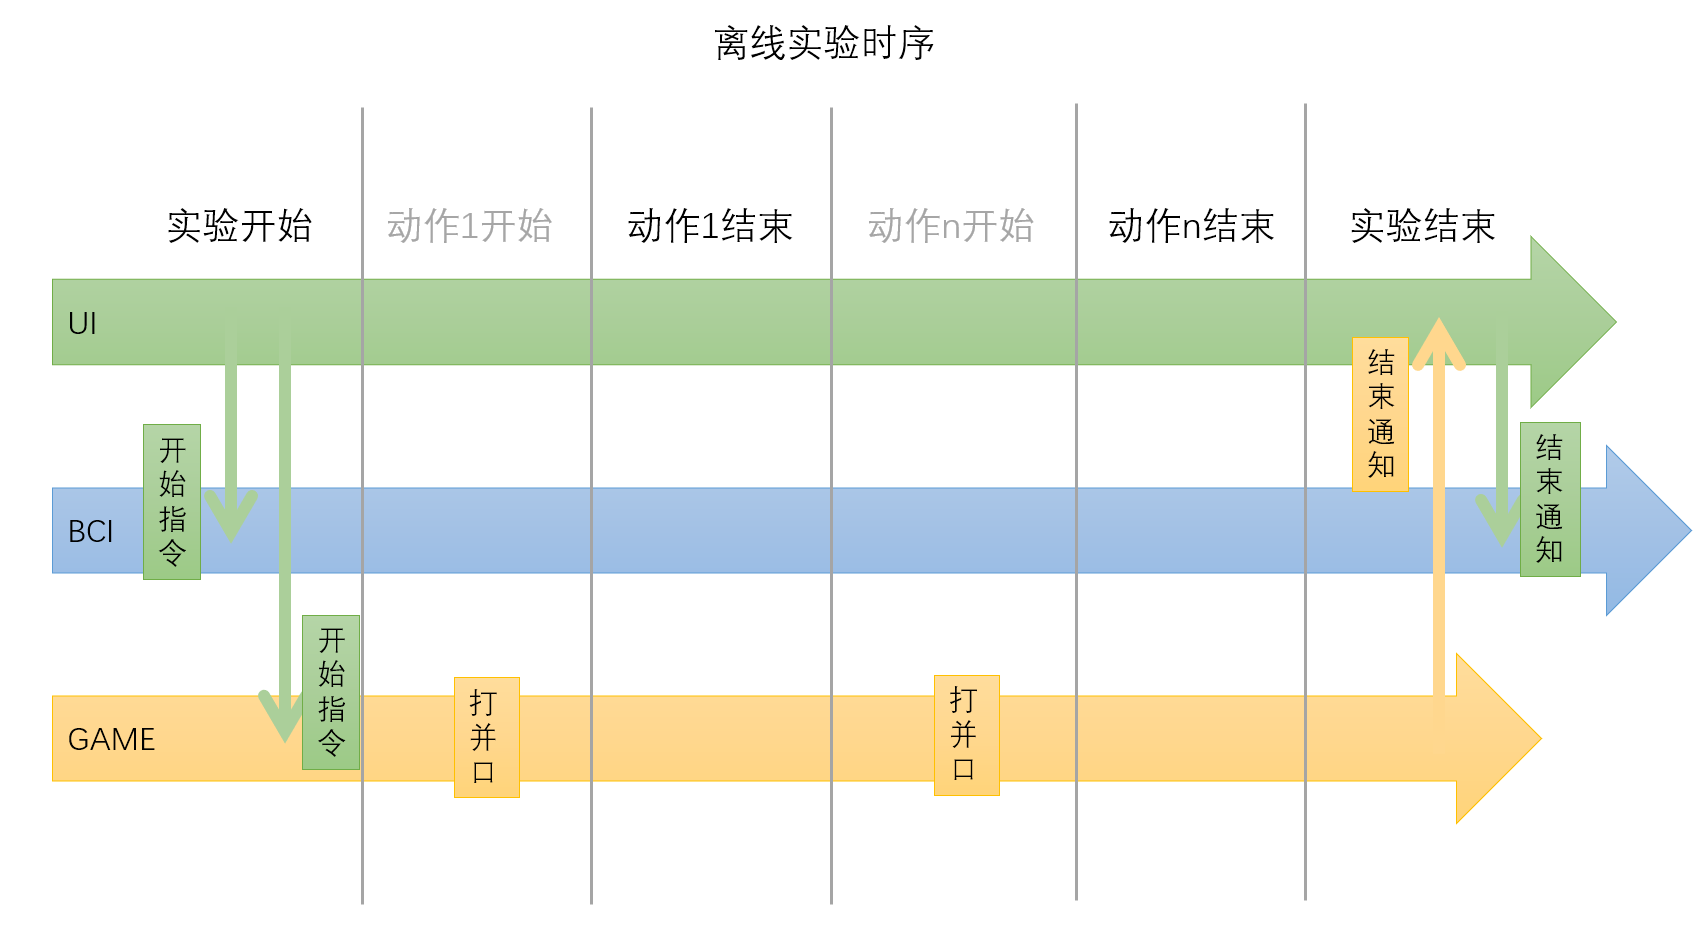
\includegraphics[width=12cm]{TimelineOffline.png}
    \caption{离线实验时序}
    \label{fig:offline}
\end{figure}

\begin{figure}[htbp]
    \centering
    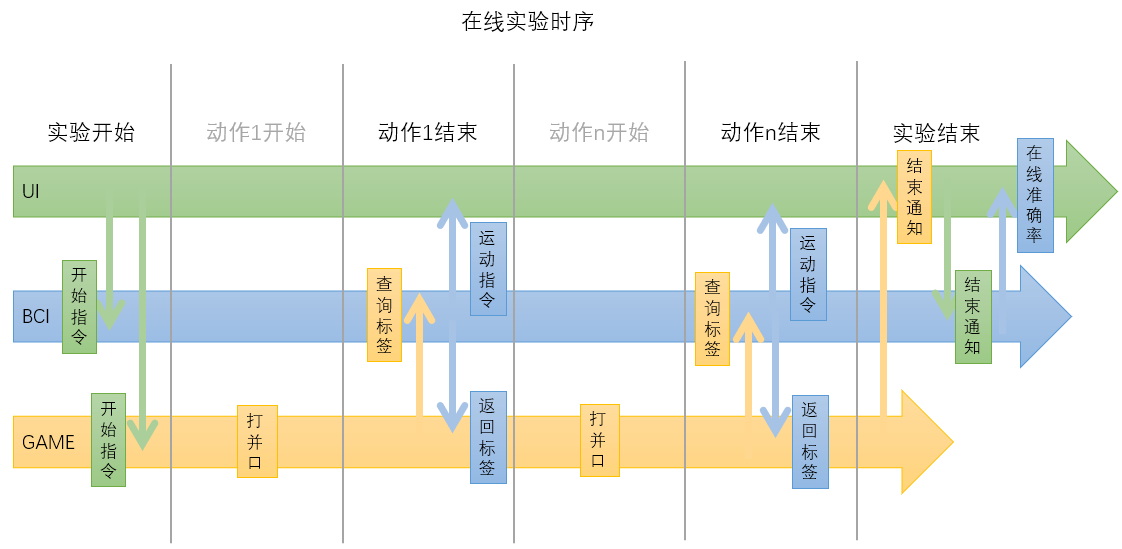
\includegraphics[width=12cm]{TimelineOnline.png}
    \caption{在线实验时序}
    \label{fig:online}
\end{figure}

% Software components
\section{软件组件}

% Table
本软件包含多个应用组件(见表\ref{tabel:components})。

\begin{table}[h!]
    \begin{center}
        \caption{组件列表}
        \label{tabel:components}
        \begin{tabular}{|l|l|l}
            \hline
            名称             & 入口文件           \\
            \hline
            主服务组件       & server.py          \\
            \hline
            后端计算组件     & local\_backend     \\
            \hline
            离线联调模拟组件 & client\_offline.py \\
            \hline
            在线联调模拟组件 & client\_online.py  \\
            \hline
            脑电设备模拟组件 & tcp\_server.py     \\
            \hline
        \end{tabular}
    \end{center}
\end{table}

% Detail
\begin{itemize}
    \item 主服务组件是软件的主体组件,负责通信管理、任务分配及日志记录功能。
    \item 后端计算组件是主要计算组件,负责脑电数据快速计算及存储。
    \item 离线联调模拟组件是调试专用组件,负责模拟离线模态下,系统其他程序的正常及异常行为。
    \item 在线联调模拟组件是测试专用组件,负责模拟在线模式下,系统其他程序的正常及异常行为。
    \item 脑电设备模拟组件是测试专用组件,用于在无脑电设备的情况下,模拟脑电设备的输出。
\end{itemize}

% Software operation
\section{软件使用}
软件由Python语言写成,在启动前需要正确配置\footnote{https://docs.python.org/3/library/python.html}{Python}运行环境,推荐的Python版本为3.6及以上,并保证本机的网络环境正确配置且支持\footnote{https://www.computerhope.com/jargon/t/tcpip.htm}{TCP/IP网络传输协议}。
软件的典型使用方法是从主服务组件启动,启动的方法是在典型Python软件运行环境中,运行以下命令即可

\begin{equation*}
    python \ server.py
\end{equation*}

软件启动后,当参数(见\ref{subsection:Params})设置正确时,软件将进入正常的待机状态。
此时软件接受TCP/IP协议格式的数据包(socket),并响应这些数据包中所包含的指令(见\ref{subsection:Socket})。

% Parameters setting
\subsection{主要参数设置}
\label{subsection:Params}

软件使用TCP/IP协议与其他软件进行通信,参数如列表\ref{table:IPparams}所示。
在启动软件之前,请对这些参数进行正确设置。

其中,``是否启动后端''是为联调测试提供的功能,当设置为$False$时将以测试模式启动,正常使用时请设置为$True$。
当设置为$False$时,软件会忽略后面计算组件的计算任务,直接给出正确结果,相应的实验数据也不会得到保存。

\begin{table}[h!]
    \begin{center}
        \caption{通信参数设置}
        \label{table:IPparams}
        \begin{tabular}{|l|l|l|l|l|}
            \hline
            参数名称     & 变量名称          & 设置文件          & 行数 & 默认值      \\
            \hline
            本机地址     & IP                & local\_profile.py & 6    & `localhost' \\
            本机端口     & PORT              & local\_profile.py & 7    & 63365       \\
            脑电设备地址 & IP\_EEG\_DEVICE   & local\_profile.py & 11   & `127.0.0.1' \\
            脑电设备端口 & PORT\_EEG\_DEVICE & local\_profile.py & 12   & 8844        \\
            是否启动后端 & USE\_BACKEND      & local\_profile.py & 10   & True        \\
            \hline
        \end{tabular}
    \end{center}
\end{table}

% API
\section{数据包指令说明}
\label{subsection:Socket}

% Classic workflow
\subsection{典型通信过程}

\begin{itemize}
    \item 心跳包通信
          \begin{itemize}
              \item $A \rightarrow B$ 心跳包
              \item $B \rightarrow A$ 回复心跳包
              \item (其中,A、B 为任意角色)
          \end{itemize}

    \item 离线游戏中,UI 要求 BCI 开始采集
          \begin{itemize}
              \item $UI \rightarrow BCI$ 开始离线采集包
              \item $BCI \rightarrow UI$ 回复包
          \end{itemize}

    \item 离线游戏中,UI 要求 BCI 进行建模
          \begin{itemize}
              \item $UI \rightarrow BCI$ 建模包
              \item $BCI \rightarrow UI$ 回复包
              \item $BCI \rightarrow UI$ 模型准确率包
          \end{itemize}

    \item 在线游戏中,GAMER 要求 BCI 估计标签
          \begin{itemize}
              \item $GAMER \rightarrow BCI$ 查询包
              \item $BCI \rightarrow GAMER$ 回复包
              \item $BCI \rightarrow GAMER$ 查询结果包
              \item $GAMER \rightarrow BCI$ 回复包
          \end{itemize}

    \item BCI 向其他人发送运行时错误
          \begin{itemize}
              \item $BCI \rightarrow Other$ 运行时错误包
              \item $Other \rightarrow BCI$ 回复包
              \item (其中,Other 为 Gamer 或 UI)
          \end{itemize}

\end{itemize}

% Socket contents
\subsection{数据包说明}

每个通信包为\footnote{https://www.json.org/json-en.html}{JSON}字典格式的二进制字符串,支持\footnote{http://www.utf-8.com/}{UTF-8}编码,字符串内容包括拉丁字母和数字,尚不包括中文。
在Python中,可以通过\footnote{https://docs.python.org/3/library/json.html}{json}包进行消息封装。

\begin{enumerate}
    \item 心跳包
          \begin{fleqn}[20pt]
              \begin{align*}
                  \begin{cases}
                      ``mode"      & : ``keepalive",     \\
                      ``timestamp" & : ``1585297645.123"
                  \end{cases}
              \end{align*}
          \end{fleqn}

    \item 开始离线采集包
          \begin{fleqn}[20pt]
              \begin{align*}\begin{cases}
                      ``mode"      & : ``Offline",                                 \\
                      ``cmd"       & : ``kaishicaiji",                             \\
                      ``shujumulu" & : ``", // \mbox{数据目录,离线数据将存在这里} \\
                      ``timestamp" & : ``1585297645.123"
                  \end{cases}\end{align*}
          \end{fleqn}

    \item 结束离线采集包
          \begin{fleqn}[20pt]
              \begin{align*}\begin{cases}
                      ``mode"      & : ``Offline",       \\
                      ``cmd"       & : ``jieshucaiji",   \\
                      ``timestamp" & : ``1585297645.123"
                  \end{cases}\end{align*}
          \end{fleqn}

    \item 建模包
          \begin{fleqn}[20pt]
              \begin{align*}\begin{cases}
                      ``mode"       & : ``Offline",                                         \\
                      ``cmd"        & : ``jianmo",                                          \\
                      ``shujumulu"  & : ``", // \mbox{数据目录,请确保目录里只包含离线数据} \\
                      ``moxingmulu" & : ``", // \mbox{模型目录,训练出的模型会存在这里}     \\
                      ``timestamp"  & : ``1585297645.123"
                  \end{cases}\end{align*}
          \end{fleqn}

    \item 模型准确率包
          \begin{fleqn}[20pt]
              \begin{align*}\begin{cases}
                      ``mode"         & : ``Offline",                                                       \\
                      ``cmd"          & : ``zhunquelv",                                                     \\
                      ``moxinglujing" & : ``", // \mbox{模型路径}                                           \\
                      ``shujulujing"  & : ``", // \mbox{数据路径,后面的准确率是根据该模型和数据计算出来的} \\
                      ``zhunquelv"    & : ``0.95", // \mbox{准确率}                                         \\
                      ``timestamp"    & : ``1585297645.123"
                  \end{cases}\end{align*}
          \end{fleqn}

    \item 开始在线采集包
          \begin{fleqn}[20pt]
              \begin{align*}\begin{cases}
                      ``mode"         & : ``Online",                                        \\
                      ``cmd"          & : ``kaishicaiji",                                   \\
                      ``moxinglujing" & : ``", // \mbox{模型路径,请确保该路径指向模型文件} \\
                      ``timestamp"    & : ``1585297645.123"
                  \end{cases}\end{align*}
          \end{fleqn}

    \item 结束在线采集包
          \begin{fleqn}[20pt]
              \begin{align*}\begin{cases}
                      ``mode"      & : ``Online",        \\
                      ``cmd"       & : ``jieshucaiji",   \\
                      ``timestamp" & : ``1585297645.123"
                  \end{cases}\end{align*}
          \end{fleqn}

    \item 在线准确率包
          \begin{fleqn}[20pt]
              \begin{align*}\begin{cases}
                      ``mode"         & : ``Online",                                                     \\
                      ``cmd"          & : ``zhunquelv",                                                  \\
                      ``moxinglujing" & : ``",                                                           \\
                                      & // \mbox{模型路径,后面的准确率是根据该模型和在线数据计算出来的} \\
                      ``zhunquelv"    & : ``0.85", // \mbox{准确率}                                      \\
                      ``timestamp"    & : ``1585297645.123"
                  \end{cases}\end{align*}
          \end{fleqn}

    \item 查询包
          \begin{fleqn}[20pt]
              \begin{align*}\begin{cases}
                      ``mode"            & : ``Query",                                                       \\
                      ``chixushijian"    & : ``3.0", // \mbox{上一个动作持续了多长时间,单位为秒,3.0是例子} \\
                      ``zhenshibiaoqian" & : ``1", // \mbox{上一个动作的真实标签,1是例子}                   \\
                      ``timestamp"       & : ``1585297645.123"
                  \end{cases}\end{align*}
          \end{fleqn}

    \item 查询结果包
          \begin{fleqn}[20pt]
              \begin{align*}\begin{cases}
                      ``mode"         & : ``QueryReply",                                \\
                      ``gujibiaoqian" & : ``1", // \mbox{上一个动作的预测标签,1是例子} \\
                      ``timestamp"    & : ``1585297645.123"
                  \end{cases}\end{align*}
          \end{fleqn}

    \item 回复心跳包
          \begin{fleqn}[20pt]
              \begin{align*}\begin{cases}
                      ``mode"      & : ``Reply",         \\
                      ``state"     & : ``keepalive",     \\
                      ``timestamp" & : ``1585297645.123"
                  \end{cases}\end{align*}
          \end{fleqn}

    \item 回复能够被正确识别的包
          \begin{fleqn}[20pt]
              \begin{align*}\begin{cases}
                      ``mode"      & : ``Reply",         \\
                      ``state"     & : ``OK",            \\
                      ``timestamp" & : ``1585297645.123"
                  \end{cases}\end{align*}
          \end{fleqn}

    \item 回复无法被正确识别的包
          \begin{fleqn}[20pt]
              \begin{align*}\begin{cases}
                      ``mode"      & : ``Reply",         \\
                      ``state"     & : ``ParseError",    \\
                      ``timestamp" & : ``1585297645.123"
                  \end{cases}\end{align*}
          \end{fleqn}

    \item 强制复位包(系统内部调用,不建议外部使用)

    \item 运行时错误-状态错误包

          代表运行状态错误,包括但不限于:
          \begin{itemize}
              \item 重复开始采集
              \item   重复停止采集
              \item   实验过程中要求建模
              \item   离线实验过程中要求查询标签
              \item   在线实验未开始时要求查询标签
          \end{itemize}

          \begin{fleqn}[20pt]
              \begin{align*}\begin{cases}
                      ``mode"      & : ``RuntimeError",  \\
                      ``type"      & : ``StateError",    \\
                      ``detail"    & : ``xxxx",          \\
                      ``timestamp" & : ``1585297645.123"
                  \end{cases}\end{align*}
          \end{fleqn}

    \item 运行时错误-文件错误包

          代表目标文件无法获取,如无法找到、无法读取等。
          \begin{fleqn}[20pt]
              \begin{align*}\begin{cases}
                      ``mode"      & : ``RuntimeError",  \\
                      ``type"      & : ``FileError",     \\
                      ``detail"    & : ``xxxx",          \\
                      ``timestamp" & : ``1585297645.123"
                  \end{cases}\end{align*}
          \end{fleqn}

    \item 运行时错误-资源忙错误包

          代表后台资源忙,操作无法运行。
          \begin{fleqn}[20pt]
              \begin{align*}\begin{cases}
                      ``mode"      & : ``RuntimeError",  \\
                      ``type"      & : ``BusyError",     \\
                      ``detail"    & : ``xxxx",          \\
                      ``timestamp" & : ``1585297645.123"
                  \end{cases}\end{align*}
          \end{fleqn}

    \item 运行时错误-未定义错误包

          代表无法事先定义,但运行时发生的错误,如内存满、关键设备断开等。
          \begin{fleqn}[20pt]
              \begin{align*}\begin{cases}
                      ``mode"       & : ``RuntimeError",  \\
                      ``type"       & : ``UnknownError",  \\
                      ``detail"     & : ``xxxx",          \\
                      ``timestamp`` & : "1585297645.123``
                  \end{cases}\end{align*}
          \end{fleqn}

\end{enumerate}

\end{document}